\subsubsection{Vuforia}
\begin{table}[H]
	\centering
	\begin{tabular}{|c|c|}
		\hline
		\multicolumn{2}{|c|}{Especificaciones de prueba}   \\ \hline
		\textbf{DISPOSITIVO}              & Moto G6 XT1925 \\ \hline
		\textbf{FECHA}                    & 2018/08/25     \\ \hline
		\textbf{VERSIÓN DE SCENEFORM SDK} & No aplica         \\ \hline
		\textbf{VERSIÓN DE Vuforia SDK}    & V7.0.50        \\ \hline
		\textbf{VERSIÓN DE ANDROID}       & V8.0.0 (Oreo)  \\ \hline
	\end{tabular}
	\captionsetup{justification=centering}
	\caption{Especificaciones de prueba Vuforia en Moto G6}
\end{table}

\textbf{Posición cardinal} \par
La aplicación necesita escanear una marca para poder dibujar el objeto, al colocar el objeto virtual se pudo apreciar con claridad desde los cuatro puntos cardinales y la vista superior. El objeto tiende a desaparecer y aparecer al mover la cámara restando realismo.

%%IMAGENES DE PUNTOS CARDINALES
\begin{figure}[H]
	\begin{minipage}{0.48\textwidth}
	\centering
		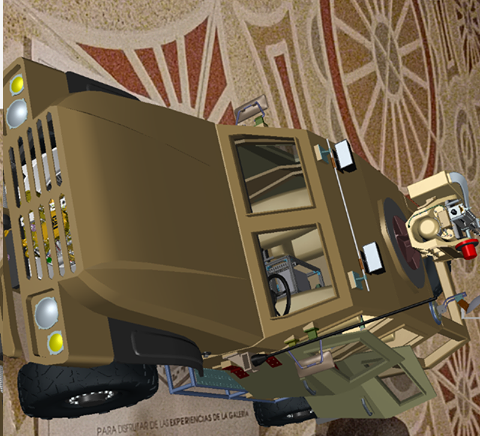
\includegraphics[width=6cm]{desarrollo/secciones/pruebas/Vuforia/img/2.png}
		\caption{Posición Norte}
		\label{fig:vuforiaNorte}
	\end{minipage}\hfill
	\begin{minipage}{0.48\textwidth}
	\centering
	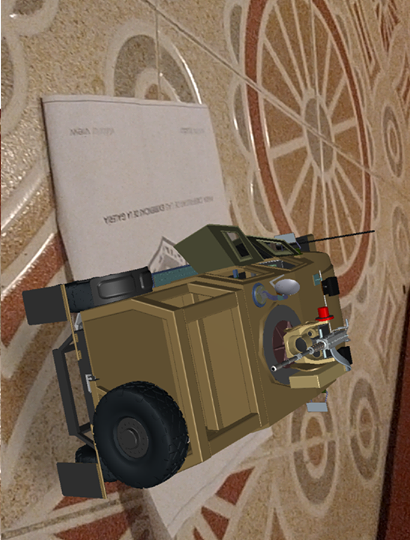
\includegraphics[width=6cm]{desarrollo/secciones/pruebas/Vuforia/img/6.png}
	\caption{Posición Sur}
	\label{fig:vuforiaSur}
	\end{minipage}\hfill
\end{figure}

\begin{figure}[H]
	\begin{minipage}{0.48\textwidth}
		\centering
		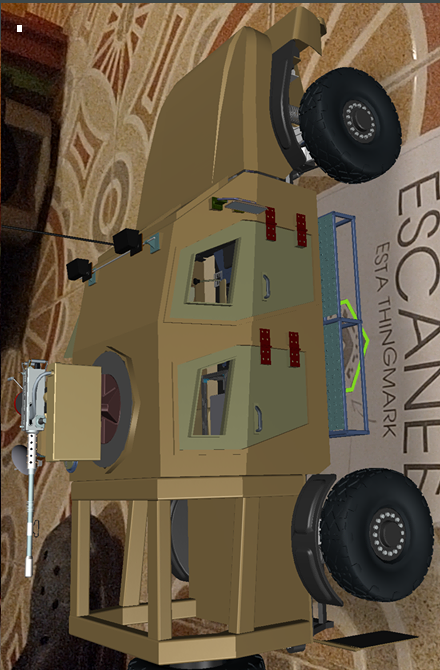
\includegraphics[width=6cm]{desarrollo/secciones/pruebas/Vuforia/img/11.png}
		\caption{Posición Este}
		\label{fig:vuforiaEste}
	\end{minipage}\hfill
	\begin{minipage}{0.48\textwidth}
		\centering
		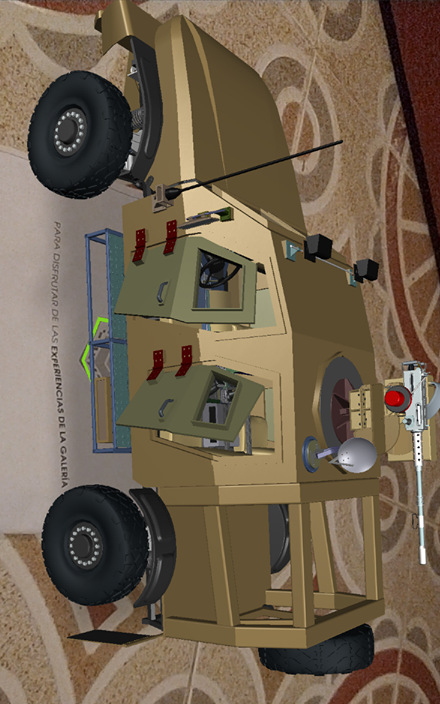
\includegraphics[width=6cm]{desarrollo/secciones/pruebas/Vuforia/img/1.png}
		\caption{Posición Oeste}
		\label{fig:vuforiaOeste}
	\end{minipage}\hfill
\end{figure}



\textbf{Tamaño relativo} \par
Al acercar o alejar la cámara el objeto virtual mantiene su tamaño original.


\begin{figure}[H]
	\begin{minipage}{0.48\textwidth}
		\centering
		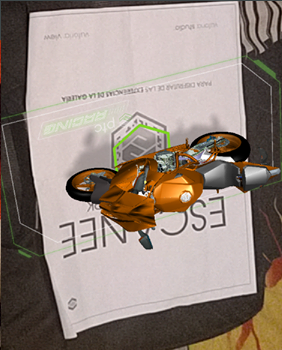
\includegraphics[width=6cm]{desarrollo/secciones/pruebas/Vuforia/img/4.png}
		\caption{Objeto visto de cerca}
		\label{fig:vuforiaCerca}
	\end{minipage}\hfill
	\begin{minipage}{0.48\textwidth}
		\centering
		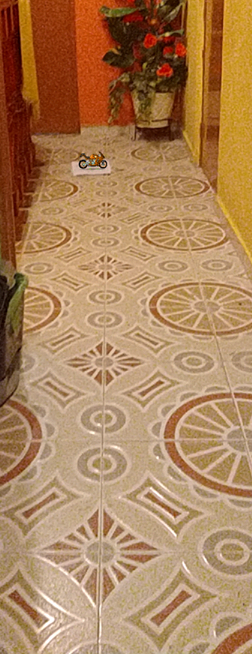
\includegraphics[width=3cm]{desarrollo/secciones/pruebas/Vuforia/img/8.png}
		\caption{Objeto visto de lejos}
		\label{fig:vuforiaLejos}
	\end{minipage}\hfill
\end{figure}

\textbf{\\Luminosidad} \par
Al poner el objeto virtual en entornos con diferente cantidad de luz, el objeto no cambia y en niveles bajos de luz el objeto desaparece.

\begin{figure}[H]
	\begin{minipage}{0.48\textwidth}
		\centering
		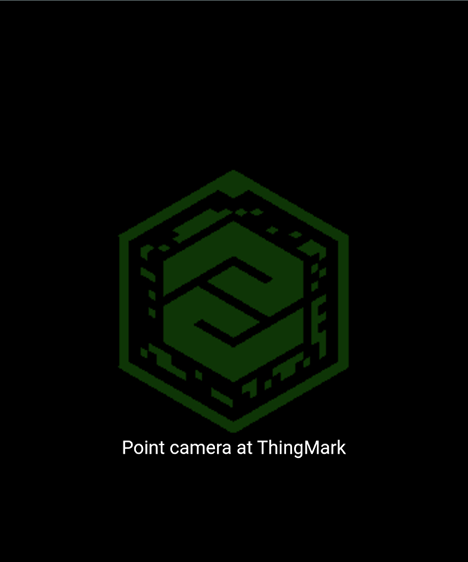
\includegraphics[width=8cm]{desarrollo/secciones/pruebas/Vuforia/img/3.png}
		\caption{Luz baja}
		\label{fig:vuforiaBaja}
	\end{minipage}\hfill
	\begin{minipage}{0.48\textwidth}
		\centering
		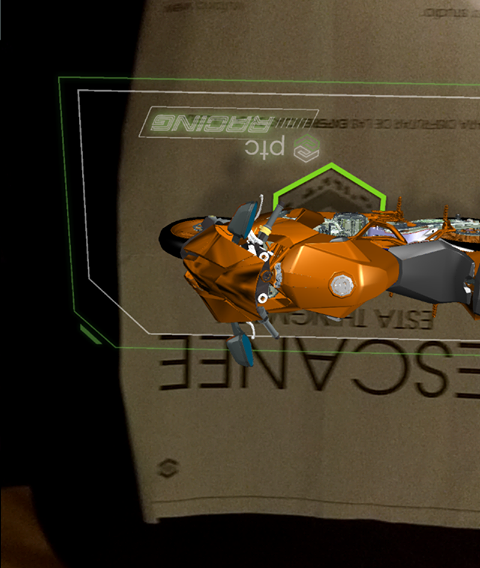
\includegraphics[width=8cm]{desarrollo/secciones/pruebas/Vuforia/img/9.png}
		\caption{Luz media}
		\label{fig:vuforiaLmedia}
	\end{minipage}\hfill
\end{figure}

\begin{figure}[H]
	\begin{minipage}{0.48\textwidth}
		\centering
		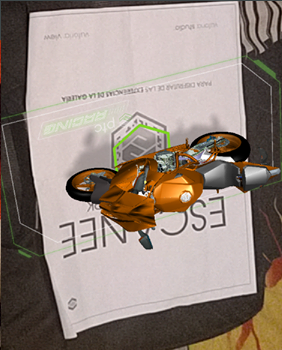
\includegraphics[width=6cm]{desarrollo/secciones/pruebas/Vuforia/img/4.png}
		\caption{Luz alta}
		\label{fig:vuforiaLAlta}
	\end{minipage}\hfill
\end{figure}

\textbf{Superficie} \par
Esta prueba no aplica en esta tecnología ya que es necesario la marca para que aparezca el objeto virtual\par

\begin{figure}[H]
	\begin{minipage}{0.48\textwidth}
		\centering
		
\includegraphics[width=8cm]{desarrollo/secciones/pruebas/Vuforia/img/12.png}
		\caption{marca de vuforia (thingmark)}
		\label{fig:vuforiaMarca}
	\end{minipage}\hfill
	
\end{figure}


\textbf{Memoria de objetos} \par
El objeto no guarda su posición, dicha posición depende del lugar en donde se coloque la marca.

\textbf{Capacidad máxima de objetos} \par
La cantidad de objetos en pantalla depende del número de marcas que se encuentren en el rango de la cámara.
